\documentclass[12pt]{article}

\usepackage{amsmath} % Math
\usepackage[normalem]{ulem} % Strike-through Text
\usepackage{graphicx} % Images
\usepackage{titlesec} % Title Configuration

\graphicspath{ {./images/} }

% Command to strike-through text in math equations
\newcommand{\cross}[1]{\text{\sout{\ensuremath{#1}}}}
% Adjust the format of subsection (#. )
\renewcommand{\thesubsection}{\arabic{subsection}.\hspace{0.2em}}
% Change subsub sections numbering to alphabetical (a))
\renewcommand{\thesubsubsection}{\thesubsection\alph{subsubsection})}
% Configure sub and subsub sections to display inline
\setcounter{secnumdepth}{3}
\titleformat{\subsection}[runin]
  {\normalfont\normalsize\bfseries}{\thesubsection}{0em}{}
\titleformat{\subsubsection}[runin]
  {\normalfont\normalsize\bfseries}{\thesubsubsection}{0.5em}{}
% Create new commands to reference exercises
\newcommand{\exercise}{\subsection{}\setcounter{subsubsection}{0}}
\newcommand{\multipartexercise}{\addtocounter{subsection}{1}\setcounter{subsubsection}{0}}
\newcommand{\exercisepart}{\subsubsection{}}

\title{
    COMP4097 Mobile Computing \linebreak
    Assignment 1
}
\author{Jonatan Juhas (19502966)}
\date{\today}

\begin{document}
\maketitle

\section*{Fundamentals of Wireless Communication}
\multipartexercise \exercisepart
Since the distances form a right angled triangle, we can use the pythagorean theorem to calculate/estimate the distance.

\begin{align*}
    c^2 &= a^2 + b^2 \\
    (6370 + \frac{h}{1000})^2 &= d^2 + 6370^2 \\
    \cross{6370^2} + \frac{2*6370*h}{1000} + (\frac{h}{1000})^2 &= d^2 + \cross{6370^2} \\
    d &= \sqrt{12.74*h + (\frac{h}{1000})^2}
    \intertext{With $(\frac{h}{1000})^2$ being negligible for $h \ll \text{earth radius}$} \\
    d &= 3.57*\sqrt{h}
\end{align*}

\exercisepart
Given Lion's Rock height of $h=495m$, the line of sight distance is $d=3.57*\sqrt{495}\approx79.43km$.
The line of sight covers all of the Hong Kong Area stretching even to Macau (see figure \ref{lionsrocklos}).

\begin{figure}[h]
    \centering
    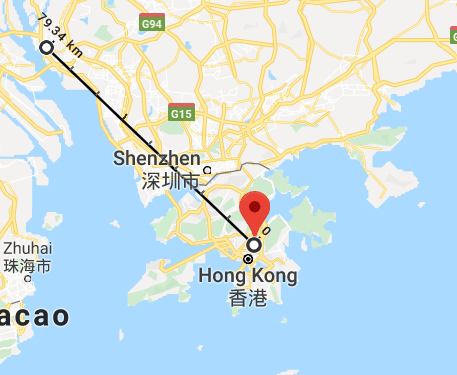
\includegraphics{lineofsight}
    \caption{Line drawn from Lion's Rock stretching 80km}
    \label{lionsrocklos}
\end{figure}

\multipartexercise \exercisepart
Assuming isotropic antennas and using the formula for free space loss we calculate the frequency of the transmission $f$:

\begin{align*}
    \frac{P_t}{P_{r_A}} &= \frac{4*\pi*f*d}{c^2} \\
    \intertext{$P_t=20mW$ $P_{r_A}=10mW$ and $d=10m$} \\
    f &= \frac{\sqrt{\frac{20mW}{10mW}*3*10^{8^2}}}{4*\pi*10m} \\
    &= \frac{7500000*\sqrt{2}}{\pi}
\end{align*}

Now substituting the frequency in our calculation for signal strength at the other mobile receiver station (B):

\begin{align*}
    \frac{20mW}{P_{r_B}} &= \frac{(4*\pi*f*20)^2}{c^2} \\
    P_{r_B} &= \frac{c^2}{(4*\pi*f*20)^2}*20 \\
    &= \frac{281250*10^9}{\pi^2*f^2} \approx 2.5mW
\end{align*}

\exercisepart
Using the previously calculated $f$ we now calculate the maximum transmission distance by regarding $d$ as variable:

\begin{align*}
    \frac{20mW}{0.125} &= \frac{(4*\pi*f*d)^2}{c^2} \\
    d &= \frac{\sqrt{(\frac{20}{0.125})*c^2}}{4*\pi*f} \\
    &= \frac{3.01975*10^8}{f} \approx 89.4427m
\end{align*}

\exercisepart
Moving the device away from the station increases the effect of multi-path propagation. The presence of reflective surfaces and objects causes the transmitted signal to arrive at the receiver displaced and causes the signal strength to fluctuate.

\section*{Advanced Wireless Transmission Techniques}
\exercise
\begin{itemize}
    \begin{minipage}{\textwidth}
    \item ASK (Amplitude Shift Keying)

    Differences in amplitude of the signal (typically depicted as different heights of the wave) can represent different bit patterns (eg. one amplitude for 1 and one for zero or 4 different amplitudes for patterns 00, 01, 10 and 11).
    \end{minipage}

    \begin{minipage}{\textwidth}
    \item BFSK (Binary Frequency Shift Keying)

    Difference in frequency of the signal (typically depicted as different widths of a wave segment) can represent different bit patterns. In this case 2 shifts are defined: one for 0 and for 1 in equal but opposite direction (reduces error rate).
    \end{minipage}

    \begin{minipage}{\textwidth}
    \item MFSK (Multiple FSK)

    Same principle as above, but uses multiple shifts in frequency. Improves the bandwidth usage but is more prone to errors.
    \end{minipage}

    \begin{minipage}{\textwidth}
    \item BPSK (Binary Phase Shift Keying)

    Differences in the phase of a signal (typically represented by moving the wave horizontally on a graph) can represent different bit patterns. 2 shifts in this case represent 0 and 1.
    \end{minipage}

    \begin{minipage}{\textwidth}
    \item MPSK (Multiple PSK)

    Same as above, but uses multiple phase shifts.
    \end{minipage}
\end{itemize}

\exercise
16-QAM can encode 16 states = $2^4$ = 4 bits. Given that we have a signal rate of 200KBaud (200000Baud or Signals per second), our data rate is $200KBaud*4=800kb=100kB$.

256-QAM can encode 256 states = $2^8$ = 8 bits. Given the same signal rate, our data rate will be $200KBaud*8=1.6Mb=200kB$.

\exercise
\textbf{FHSS (Frequency Hopping Spread Spectrum)} rapidly changes carries among many frequency channels in a way both transmitter and receiver always choose equally (pseudo-random sequence). In this way jamming becomes difficult, since the adversary would have to either know the sequence or jam a wide array of channels at once hoping to hit the right ones. Similar is true for intercepting the signals.

\textbf{DSSS (Direct Sequence Spread Spectrum)} uses a similar pseudo-random sequence to encode a single bit into several bits (using xor). In this case jamming can become difficult, as jamming several bits of a signal in a row requires the adversary to jam the amount*constant. Security-wise, this encoding is similar to a stream cipher.

\section*{Principles and Standards of Wireless LANs \& Management}
\exercise
The hidden node problem is based around the fact that multiple nodes can be connected to an access point without being in range within each other (they themselves cannot communicate with each other).

Medium access control is used to make sure messages aren't sent at the same time. \textbf{CSMA/CD} can be summed up as first looking if anyone else is transmitting (CS), then while transmitting itself detecting collisions (CD). If a collision is detected, a jamming signal is sent, with the transmission being interrupted and repeated after a random wait period.

With \textbf{CSMA/CA} the node uses a similar method but, since after the transmission has started \textbf{is itself unable to reliably determine if anyone else is transmitting} (reason why CSMA/CD cannot be used), attempts to transmit the entire message and then waits for confirmation. If no confirmation (including data checksum) is received, the message is considered to have been lost.

\exercise
\textbf{RTS/CTS} (Request to Send/Clear to Send) can be used as an additional measure to resolve the hidden node problem. Since the node has to first request "permission" to send data, nodes within reach as well as the receiver will know it wants to send and can act appropriately (senders will wait, receiver can decide to grant the request or accept other requests instead). A major disadvantage is, that this exchange slows down the transmission, since now 2 more messages have to be exchanged for every message/frame. This increases the transmission time.

\exercise
The IEEE 802.11n standard improves upon the g-one by using multiple antennas and signals instead of one. This technology is called MIMO - multiple input, multiple output.

IEEE 802.11ac further improves speed by extending concepts embraced by the n-standard. Supporting simultaneous transmission on both the 2.4GHz, as well as the 5GHz bands, it offers transmission speeds of up to 1300Mb per second.

\exercise
The WEP standard "features" several flaws within its specification.
The first one being, that there are \textbf{no key management requirements} within it. This leads to the same keys being potentrally used for a long time, which can result in the traffic being decrypted once such a key is cracked, as well as sharing keys among clients which can be used by one malicious client trying to decrypt other's transmissions.

A second crucial vulnerability is the \textbf{IV (Initialization Vector)} being too small and sent in clear text. It consists of only 24bits which make up for $\approx$16million different streams. Given the way in which they are chosen is also not specified (often starts at 0 incrementing with each packet and re-rolling at the end or randomly chosen), the possibility of the same IV being used more than once is very high. Once a stream for a particular IV is found, the adversary can decrypt any packet sent using this IV.

There are other issues within this standard such as the usage of weak algorithms, but such issues are time relevant. That is to say, given enough time any algorithm has the potential to become obsolete or inadequate and has to be replaced by a more sophisticated version. The \textbf{lack of specification} within the standard is the most damaging aspect of WEP and is the reason why today, specifications try to cover as many areas as deemed appropriate, so that security is enforced rather than optionally ignored.

\end{document}
